\documentclass[12pt]{scrartcl}
 
\usepackage{graphicx}
\usepackage[english,german]{babel}
 
\begin{document}

\begin{titlepage}
	\centering
	{\scshape\LARGE Ostfalia Hochschule \par}
	\vspace{1cm}
	{\scshape\Large EKdI-Projekt\par}
	\vspace{1.5cm}
	{\huge\bfseries Pflichtenheft\par}
	\vspace{2cm}
	{\Large\itshape Martin Krause 70478294, Tom Strunz 70476813, Patricia Weber 70477439, Kristin Altmann 70476503\par}
	\vfill
	supervised by\par
	Prof. \textsc{Jensen}

	\vfill

% Bottom of the page
	{\large \today\par}
\end{titlepage}


\tableofcontents
\newpage


\section{Zweck und Ziel}
Es soll ein Programm in Java >= 11, mit Open JDK, entwickelt werden, welches mit dem Aufrufen des \glqq Lies.java\grqq Java-Programms den Inhalt einer beliebigen Webseite vorlesen soll. Dabei muss beachtet werden das die nicht dargestellten Bestandteile, zum Beispiel Tags und Metadaten, nicht vorgelesen werden sollen. Dieses Programm soll entwickelt werden um zum Beispiel Personen mit Sehbehinderung Webseiten hinter URLs inhaltlich zeigen zu können. Dieses Pflichtenheft basiert auf dem dazugehörigem Lastenheft und beinhaltet alle Zwecke und Ziele des Lastenhefts außer sie werden ausgeschlossen.

\section{Abgrenzung}
Das Programm soll kein Graphic User Interface (GUI) enthalten und dem Programm wird es ebenfalls fast nur möglich sein Deutsche Webseiten vorzulesen, aufgrund von den auf Deutsch eingelesenen Silben. Das Proramm wird unter Windows geschrieben und getestet.

\section{Begriffe}
\begin{itemize}
    \item 'URL': Adressierung der vorzulesenden Website
    \item 'vorlesen': Abspielen von wav-Dateien, die den Worten des Texts entsprechen
    \item 'Text': der Haupttext auf der Website
    \item 'Start': Beginn/ Fortsetzen des Vorlesens
    \item 'Stopp': Unterbrechen des Vorlesens
    \item 'parsen': Zerlegen und umwandeln für eine Weiterverarbeitung
    \item 'Silbe': eine Buchstabenkombination einer Silbe im grammatikalischen Sinne zuweisbar ist, gilt dies als Silbe. Da nicht alle Silben der deutschen Sprache eingesprochen werden können, werden Buchstaben, die nicht                 einer Silbe zugeordnet werden können, als Silbe aus nur einem Buchstaben betrachtet.
\end{itemize}

\section{Soll-Stand}
Was soll erreicht werden?
Das Programm soll einen Text von einer Website, deren URL dem Programm übergeben wurde, einlesen und dann vorlesen.
Wie soll das erreicht werden?
Das Programm besteht im Wesentlichen aus zwei Teilen: dem Einlesen und dem Vorlesen. Beim Einlesen werden zuerst Daten von der Website abgegriffen und der HTML-Code geparst. Für das Vorlesen müssen Start, Stopp, das Trennen des Texts in Silben und das Wandeln der Silben in gesprochene Sprache. Die Silben müssen dementsprechend noch eingesprochen werden.
Was kann noch erreicht werden?
Es könnte eine Warnungen ausgegeben werden, wenn der Text wahrscheinlich nicht auf Deutsch ist, zu lang ist oder die wav-Dateien, die zum Vorlesen nötig sind, nicht gefunden werden. Außerdem könnte der vorgelesene Text ausgegeben werden.


\subsection{Funktionen}

LF1: Beim Programmstart, wird eine URL übergeben.
-- java Lies www.ostfalia.de
\begin{figure}[hp!]
 \centering
 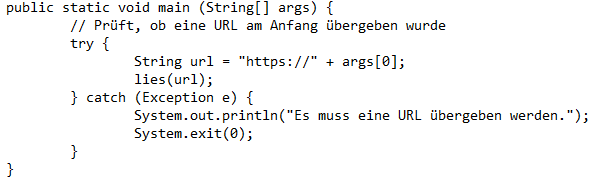
\includegraphics[width=1.0\textwidth]{res/LF1}
 \caption{LF1}
 \label{fig: fig1}
\end{figure}
~

\newpage

LF2: Das Vorlesen kann gestartet werden und beliebig pausiert und wieder weitergespielt werden. Außerdem kann das Programm beliebig beendet werden.
\begin{figure}[hp!]
 \centering
 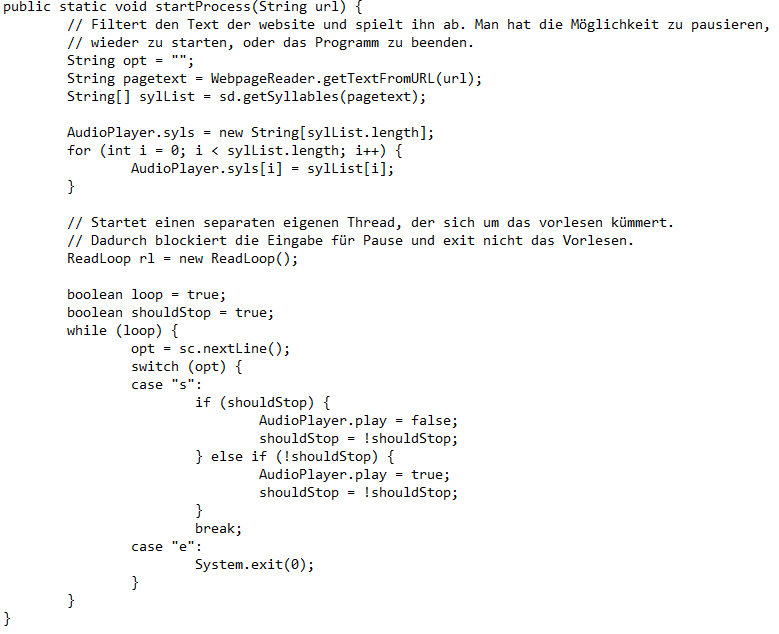
\includegraphics[width=1.0\textwidth]{res/LF2}
 \caption{LF2}
 \label{fig: fig2}
\end{figure}
~

\newpage

LF3: Der Text aus einer Webseite wird herauskopiert.
\begin{figure}[hp!]
 \centering
 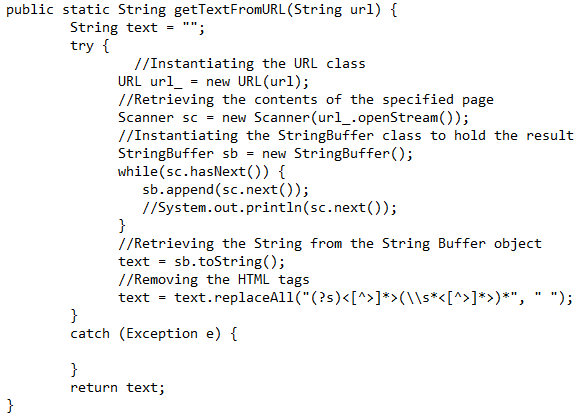
\includegraphics[width=0.8\textwidth]{res/LF3}
 \caption{LF3}
 \label{fig: fig3}
\end{figure}
~

\newpage

LF4: Der Text wird geparst und die Steuerzeichen werden heraus gefiltert.
\begin{figure}[hp!]
 \centering
 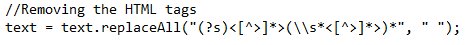
\includegraphics[width=0.6\textwidth]{res/LF4}
 \caption{LF4}
 \label{fig: fig4}
\end{figure}
~

\newpage

LF5: Der Text wird in Silben bzw. einzelne Buchstaben aufgeteilt.
\begin{figure}[hp!]
 \centering
 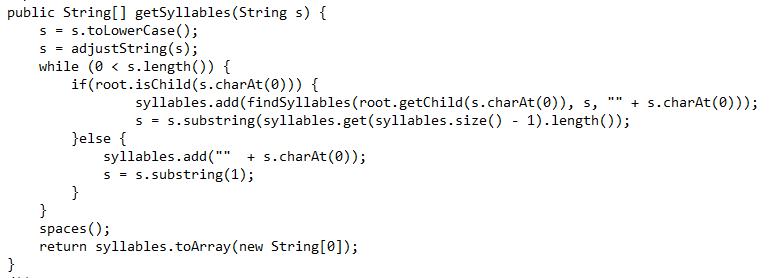
\includegraphics[width=0.8\textwidth]{res/LF5}
 \caption{LF5}
 \label{fig: fig5}
\end{figure}
~

\newpage

LF6: Die Silben werden nacheinander abgespielt.
\begin{figure}[hp!]
 \centering
 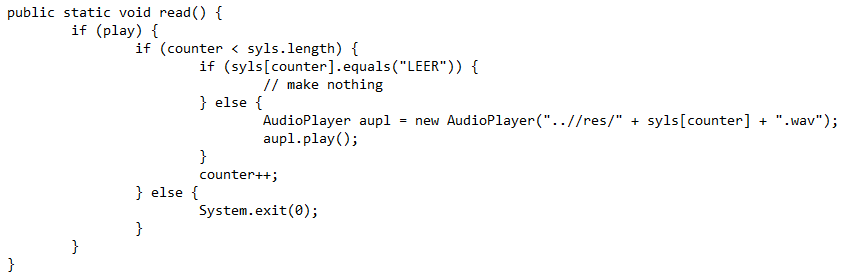
\includegraphics[width=0.9\textwidth]{res/LF6}
 \caption{LF6}
 \label{fig: fig6}
\end{figure}
~
	
\newpage
	
LF7: Der Thread kümmert sich in einer Endlosschleife um das Vorlesen nach einer bestimmten kurzen Pause.
\begin{figure}[hp!]
 \centering
 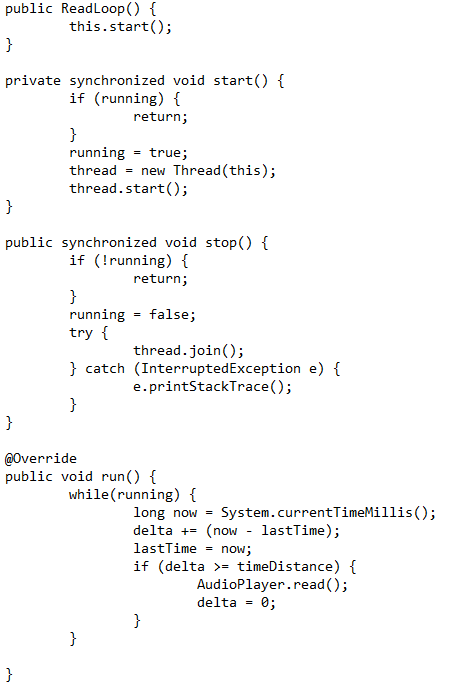
\includegraphics[width=0.6\textwidth]{res/LF7}
 \caption{LF7}
 \label{fig: fig7}
\end{figure}
~

\newpage

\subsection{Daten}
\begin{itemize}
	\item LD1: Die ersten Daten mit dem das Programm konfrontiert wird ist die übergebene URL.
	\item LD2: Mit Tastatureingabe \glqq l\grqq beginnt das Programm mit dem Vorlesen.
	\item LD3: Mit Tastatureingabe \glqq s\grqq kann das Vorlesen gestoppt und wieder weitergespielt werden.
	\item LD4: Mit Tastatureingabe \glqq e\grqq kann das Programm beendet werden.
	\item PD1: Die URL wird als String gespeichert.
	\item PD2: Der Text der Webseite wird als String gespeichert.
	\item PD5: Die Silben werden als Strings in einem Array gespeichert.
	\item PD6: Alle Silben sind als wav-Dateien dem Programm beigelegt, um abgespielt werden zu können.
\end{itemize}


\subsection{Regeln}

\begin{itemize}
	\item PR1: Das Programm soll mit dem Aufruf java Lies \glqq URL\grqq den Inhalt einer beliebigen URL vorlesen. Falls keine URL übergeben wurde, wird eine Exception geworfen und der Nutzer wird darüber informiert.
	\item LR2: Andere Libraries als die der Oracle JDK oder OpenJDK dürfen nicht verwendet werden.
	\item LR3: Der Aufruf externer Services oder Programme zum Vorlesen ist nicht erlaubt.
	\item LR4: Nicht dargestellte Bestandteile einer Website, d.h. Tags oder Metadaten, dürfen nicht vorgelesen werden.
	\item PR2: Falls eine nicht bekannte Webseite aufgerufen werden soll, wird eine Exception geworfen und der Nutzer wird darüber informiert.
	\item PR3: Falls eine nicht vorhandene Ton-Datei abgespielt werden soll, wird eine Exception geworfen und der Nutzer wird darüber informiert.
\end{itemize}

\subsection{Nichtfunktionale Anforderungen}

\begin{itemize}
	\item NA1: Das Programm soll von Personen mit Sehbehinderung bedient werden können.
\end{itemize}

\section{Dokumentenhistorie}

\begin{enumerate}
	\item | Martin Krause | Ersterstellung | 06.12.21
	\item | Kristin Altmann | Bearbeitung Punkt 1,2  | 06.12.21
	\item | Tom Strunz | Begriffe, Soll-Stand überarbeitet | 13.12.21
	\item | Patricia Weber | Regeln, Nichfunktionale Anforderungen | 13.12.21
	\item | Martin Krause | Deckblatt, Inhaltsverzeichnis, Funktionen bearbeitet | 13.12.21
	\item | Martin Krause | Funktionen grafisch eingefügt | 19.01.22
\end{enumerate}
 
\end{document}
